\documentclass{report}[a4paper,12pt] %article,book,report

\usepackage{header}

\begin{document}
  \pagenumbering{arabic}
  \maketitle %Insert Title
  \newpage %Break Page
  \tableofcontents

%\part{One}
\chapter{Basics} %book,report only
\section{Introduction}
This is the introduction section.
\href{http://www.latex-tutorial.com}{LaTeX-Tutorial} is being followed.
\href{https://www.overleaf.com/learn}{Overleaf} also has good guide.

\paragraph*{Latex} allows you to typeset document quickly using smart markup language.
There are many plugins (packages) available to enhance functionality.

\subsection{Subsection}
This is a subsection.  
Organisation of Content is done in this manner, \href{https://www.overleaf.com/learn/latex/Sections_and_chapters}{guide}.

\subsubsection{Sub Subsection}
This is a sub-subsection.

\paragraph{Paragraph} 
This is a Paragraph.

\subparagraph{Sub Para}
This is a Sub Paragraph

\section{Features}

\subsection{Math}

\paragraph{Equations}
Equations Package Example.
\begin{equation}
  f(x) = x^2
\end{equation}

\paragraph{Embedding}

This formula $f(x) = x^2$ is an embedding.

\paragraph*{Double Line}

\begin{equation*}
  1 + 2 = 3 
\end{equation*}

\begin{equation*}
  1 = 3 - 2
\end{equation*}

\begin{align*}
  1 + 2 &= 3\\
  1 &= 3 - 2
\end{align*}

\paragraph{Fractions}

\begin{align*}
  f(x) &= x^2\\
  g(x) &= \frac{1}{x}\\
  F(x) &= \int^a_b \frac{1}{3}x^3
\end{align*}

Refering to Foot Note\footnote{\label{myfootnote}Tutorial footnote}.

\subsection{Formatting}
Various \hypertarget{sen:formatopts}{Formattings} are Available. There various options for \href{https://www.overleaf.com/learn/latex/Font_sizes%2C_families%2C_and_styles}{Styling}.

\subsubsection{Styles}
\paragraph{Basic} Formatting Options using Tags.
\begin{enumerate}
  \item Styles
  \begin{enumerate}
    \item \textbf{Bold}
    \item \textit{Italics}
    \item \underline{Underline}
    \item \emph{Emphatic} (Prefer over Italics, differnt in environments)
    \item \textsl{slanted}
    \item \textsc{small caps}
    \item \textmd{medium}
    \item \textup{upright}
  \end{enumerate}
  \item `Single Quote'
  \item ``Double Quote''
  \item Special Chars, \verb|*`-$&|
  \item Space <\space>
  \item Size
  \begin{enumerate}
    \item \small small or \tiny tiny
    \item \normalsize normalsize
    \item \large large or \Large Large
    \item \huge huge or \Huge Huge
  \end{enumerate}
\end{enumerate}

\paragraph{Document} Set Stlyes (Point till end)
\begin{enumerate}
  \item \verb|\sffamily| , Revert: \verb|\rmfamily|
  \item \verb|\texttt| 
\end{enumerate}

\subsubsection{Spacing} 
Spacing can be \href{https://www.overleaf.com/learn/latex/Articles/How_to_change_paragraph_spacing_in_LaTeX}{changed} for a section or point onwards.

\paragraph{Double spacing}
\doublespacing
\lipsum[1]

\paragraph{Half spacing}
\onehalfspacing
\lipsum[1]

\begin{spacing}{2.5}
\paragraph{Spacing} `environment' allows changes for part of text.
Spacing can be specified in environment.
\begin{enumerate}
  \item Number eg. 2.5
  \item singlespace,doublespace,onehalfspace
  \item \verb|\vspace{10pt}| or \verb|\hspace{2cm}| to add space.
\end{enumerate}

\lipsum[1]
\end{spacing}

\paragraph{Normal spacing}
\lipsum[1]

\subsubsection{Colors}
Coloring can be \href{https://www.overleaf.com/learn/latex/Using_colours_in_LaTeX}{done} using \href{https://mirrors.sjtug.sjtu.edu.cn/ctan/macros/latex/contrib/xcolor/xcolor.pdf}{xcolor} package.

\paragraph{Usage}
\begin{enumerate}
  \color{teal}
  \item Changed color to teal inside begin block.
  \item Done only for List Section.
  \item Single \textcolor{Sepia}{word} color change.
  \item Background Color change Eg. \colorbox{BurntOrange}{orange background}
  \item \verb|\pagecolor{gray}| sets Page Color.
\end{enumerate}

{\color{RubineRed} \rule{\linewidth}{0.5mm}}
Can also be used to draw colored rulers. 

\definecolor{mypink2}{RGB}{219, 48, 122}
\paragraph{Custom} colors can be defined and \textcolor{mypink2}{used}.

\begin{minted}{tex}
  \definecolor{mypink1}{rgb}{0.858, 0.188, 0.478}
  \definecolor{mypink2}{RGB}{219, 48, 122}
  \definecolor{mypink3}{cmyk}{0, 0.7808, 0.4429, 0.1412}
  \definecolor{mygray}{gray}{0.6}
\end{minted}

\subsubsection{Alighnment}
\paragraph{Alignment} Can be done using align block. 
\verb|*| Indicates not to put number for that Section.

\begin{align*}
  \text{Left Align}\\
  \text{Right aligned}
\end{align*}

I'm referring to footnote again using \verb|\ref| \ref{myfootnote}.

\subsection{References}
There are many ways to reference. We use package `hyperref'.
\begin{enumerate}
  \item Direct URL \url{https://www.overleaf.com/learn/latex/Hyperlinks}
  \item Hyper Link: \href{https://www.overleaf.com/learn/latex/Hyperlinks}{Hyperlink Guide}
  \item Link to Sentence
  \item File Link: \href{run:../../presentation/beamer/tutorial.tex}{Beamer Example}
  \item Reference to a label \ref{lst:bullet}.
  \item Page Reference: \pageref{fig:coffee}
  \item Word or \hyperlink{sen:formatopts}{sentence} in your document.
\end{enumerate}

\subsection{Highlights}
\href{https://mirror.niser.ac.in/ctan/macros/latex/contrib/tcolorbox/tcolorbox.pdf}{tcolorbox} and awesomebox (xelatex only) allows you to create
fance boxes. Import tcolor \href{https://tex.stackexchange.com/questions/238303/tcolorbox-incompatibe-with-color-package}{before} xcolor.

\subsubsection{Basic}
\begin{tcolorbox}
  This is a \textbf{tcolorbox}.
\end{tcolorbox}

\begin{tcolorbox}[colback=blue!25!white,colframe=green!75!black,title=Box Heading]
  Upper Text
  \tcblower
  Lower Text.
\end{tcolorbox}

\subsubsection{Define}
\paragraph{tcolorbox} allows you to define own boxes and then use them.

\newtcolorbox{info}[1]{colback=blue!5!white,
colframe=blue!75!black,fonttitle=\bfseries,
title={#1}}

\begin{info}{Info Title}
This is my own box of type info ..
\end{info}

\subsubsection{Commands}
%textmarker style from colorbox doc
\tcbset{textmarker/.style={%
        enhanced,
        parbox=false,boxrule=0mm,boxsep=0mm,arc=0mm,
        outer arc=0mm,left=6mm,right=3mm,top=7pt,bottom=7pt,
        toptitle=1mm,bottomtitle=1mm,oversize}}

% define new colorboxes
\newtcolorbox{hintBox}{textmarker,
    borderline west={6pt}{0pt}{yellow},
    colback=yellow!10!white}
\newtcolorbox{importantBox}{textmarker,
    borderline west={6pt}{0pt}{red},
    colback=red!10!white}
\newtcolorbox{noteBox}{textmarker,
    borderline west={6pt}{0pt}{green},
    colback=green!10!white}

% define commands for easy access
\newcommand{\note}[1]{\begin{noteBox} \textbf{Note:} #1 \end{noteBox}}
\newcommand{\warning}[1]{\begin{hintBox} \textbf{Warning:} #1 \end{hintBox}}
\newcommand{\important}[1]{\begin{importantBox} \textbf{Important:} #1 \end{importantBox}}

\note{This is a Note ..}
\warning{This is a warning ..}
\important{This is an important info !!}

\begin{noteBox}
  This is a Note in environment
\end{noteBox}

\subsubsection{Alert Message}

Simple package \href{https://www.ctan.org/pkg/alertmessage}{alertmessage} to give below
functionality and nothing else ..

\alertinfo{This is info.}
\alertsuccess{Success message}
\alertwarning{Warning Message}
\alerterror{Error Message ..}

\newpage
\subsection{Images}

\paragraph{Placement Specifiers} control \href{https://www.overleaf.com/learn/latex/Positioning_images_and_tables#The_figure_environment}{placement} of image and tables.
\verb|h!| indicates to place image where it appears. Try `New Page' if it is not being honored.

Images can also be in multiple folders. \verb|\graphicspath{ {./images1/}{./images2/} }|.
Size, rotation can be \href{https://www.overleaf.com/learn/latex/Inserting_Images}{tuned} as well.

\paragraph{Single}

Figure \ref{fig:sailboat} shows a boat. %Refers Label

\begin{figure}[h]
  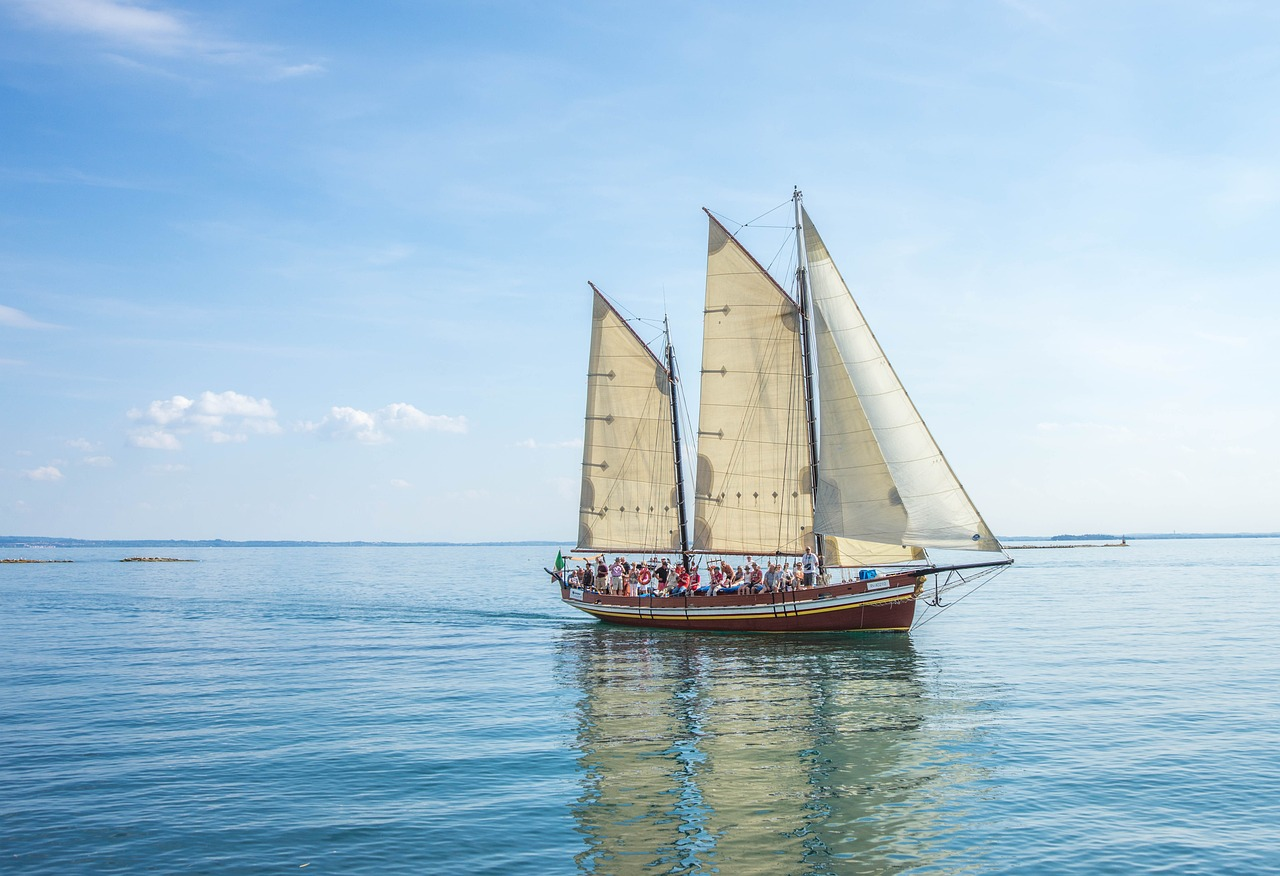
\includegraphics[width=\linewidth,scale=1.5]{boat.jpg}
  \caption{Sail Boat.}
  \label{fig:sailboat} %Invisible Used for Reference
\end{figure}

\newpage
\paragraph{Multiple}
Figure \ref{fig:coffee} shows how to place image side by side.

\subparagraph{Images aligned} next to each other, their widths are both set to \textbf{0.4}, yet they fill up the whole space.
You should always set this value to .1 less than you expect.

\begin{figure}[h!]
  \centering
  \begin{subfigure}[b]{0.4\linewidth}
    
\includegraphics[width=\linewidth]{coffee.jpg}
    \caption{Coffee.}
  \end{subfigure}
  \begin{subfigure}[b]{0.4\linewidth}
    
\includegraphics[width=\linewidth]{coffee.jpg}
    \caption{More coffee.}
  \end{subfigure}
  \caption{Two Coffies}
  \label{fig:coffee}
\end{figure}

If you want to align three images next to each other,
you should consecutively add three subfigures, each with a \verb|.2\linewidth|


\paragraph{Cluster}
Figure \ref{fig:coffee3} shows how to place cluster of images.

\subparagraph{Notice} images are Numbered Automatically.

\begin{figure}[h!]
  \centering
  \begin{subfigure}[b]{0.2\linewidth}
    
\includegraphics[width=\linewidth]{coffee.jpg}
     \caption{Coffee.}
  \end{subfigure}
  \begin{subfigure}[b]{0.2\linewidth}
    
\includegraphics[width=\linewidth]{coffee.jpg}
    \caption{Tasty coffee.}
  \end{subfigure}
  \begin{subfigure}[b]{0.2\linewidth}
    
\includegraphics[width=\linewidth]{coffee.jpg}
    \caption{More coffee.}
  \end{subfigure}
  \begin{subfigure}[b]{0.5\linewidth}
    
\includegraphics[width=\linewidth]{coffee.jpg}
    \caption{Too much coffee.}
  \end{subfigure}
  \caption{Coffee Cluster}
  \label{fig:coffee3}
\end{figure}

\subsection{Tables}

\paragraph{Useful} Resources
\begin{align*}
  \href{https://tableconvert.com/latex-generator}{Table Generator}\\
  \href{https://www.tablesgenerator.com/latex_tables}{Book Table Generator}\\
  \href{https://latex-tutorial.com/tutorials/tables/}{Tutorial}
\end{align*}

\paragraph*{Packages} for Tables
\begin{enumerate}
  \item Prettify your tables using the booktabs package.
  \item Make your tables span multiple pages with the longtable package
  \item Display your tables in landscape using the rotating package  
\end{enumerate}

\begin{table}[!h]
  \centering
  \caption{Basic Table}
  \begin{tabular}{|l|l|}
  \hline
      \textbf{Heading 1} & \textbf{Heading 2} \\ \hline
      Hello & World \\ \hline
  \end{tabular}
  \label{tab:basic}
\end{table}

\begin{table}[h!]
  \begin{center}
    \caption{Alighned Table}
    \label{tab:alighned}
    \begin{tabular}{l|c|r} % <-- Alignments: 1st column left, 2nd middle and 3rd right, with vertical lines in between
      \textbf{Value 1} & \textbf{Value 2} & \textbf{Value 3}\\
      $\alpha$ & $\beta$ & $\gamma$ \\
      \hline
      1 & 1110.1 & a\\
      2 & 10.1 & b\\
      3 & 23.113231 & c\\
    \end{tabular}
  \end{center}
\end{table}

\begin{table}[h!]
  \centering
  \caption{Book Table}
  \label{tab:book}
  \begin{tabular}{@{}lcr@{}} %<-- Left, Center, Right
    \toprule % <-- Toprule here
    \textbf{Value 1} & \textbf{Value 2} & \textbf{Value 3}\\
    $\alpha$ & $\beta$ & $\gamma$ \\
    \midrule % <-- Midrule here
    1 & 1110.1 & a\\
    2 & 10.1 & b\\
    3 & 23.113231 & c\\
    \bottomrule % <-- Bottomrule here
  \end{tabular}
\end{table}

\subsection{Lists}
Lists are easy to \href{https://www.overleaf.com/learn/latex/Lists}{create}.

\subsubsection{Bullets}
\begin{itemize}
  \label{lst:bullet}
  \item List entries start with the \verb|\item| command.
  \item Individual entries are indicated with a black dot, a so-called bullet.
  \item The text in the entries may be of any length.
  \item Below is an example of Nested List.
  \begin{itemize}
    \item Sub List 1
    \item \lipsum[1]
    \item Sub List 3
  \end{itemize}
\end{itemize}

\subsubsection{Ordered}
This is an example of Ordered Lists.

\begin{enumerate}[label=(\roman*)]
  \label{lst:order}
  \item Latex is much more powerful than Markdown.
  \item It has lot more options as compared to markdown.
  \item Markdown syntax is simple but also limited.
  \begin{description}
    \item[Note:] This allows me to add such sections.
    \item[Tip!] Most of the complex Syntax is handled via IDE.
  \end{description}
\end{enumerate}

\subsubsection{Custom}
\paragraph{Custom} bullet points can be set. Many \href{https://latex-tutorial.com/bullet-styles/}{Styles} are available.
Package `enumitem' helps customize it for Ordered List \ref{lst:order} as well.
\begin{itemize}
  \label{lst:format}
  \item[--] Dash
  \item[$-$] Dash
  \item[$\ast$] Asterisk
\end{itemize}

\vspace{10pt}

\subsubsection{No Label}
\paragraph{Without Label} Lists can also be created using `description' environment.

\begin{description}
  \item This is an entry \textit{without} a label.
  \item[Something short] A short one-line description.
  \item[Something long] A much longer description. \lipsum[1]
\end{description}

\chapter{Advanced}
\section{Code}
\paragraph{Minted} Packages allows to format and display Code. Detailed \href{https://mirror.niser.ac.in/ctan/macros/latex/contrib/minted/minted.pdf}{guide}.

\begin{enumerate}
  \item Code Snippet \ref{code:snippet} and File. \ref{code:file}
  \item Code can also be given inline \verb|\mintinline{c}|fmt.Println("Hello")|| (Not Working)
\end{enumerate}

\subsubsection{Snippet}
\begin{listing}[h]
  \begin{minted}[linenos,bgcolor=lime]{Python}
    def hello_world():
    print("Hello floating World!")
  \end{minted}
  \caption{Code Snippet}
  \label{code:snippet}
\end{listing}

\subsubsection{Beamer Latex}
\label{code:file}
\paragraph{Code} file example for Minted.
\inputminted{tex}{../../presentation/beamer/tutorial.tex} 

\subsubsection{Basic}
\begin{verbatim}
  Text enclosed inside \texttt{verbatim} environment 
  is printed directly 
  and all \LaTeX{} commands are ignored.
\end{verbatim}

\section{Editor}
Tool of choice is \href{https://github.com/James-Yu/LaTeX-Workshop}{Latex Workshop} in Vscode.
\subsection{Hotkeys}
\begin{itemize}
  \item Use Insert Snippet to Access Surround Settings.
  \item SyncTex from Cursor can be used to focus current PDF Location where edit is Happening.
  \item Auto Complete is Triggered both on \verb|\|
  \item Other Auto Completions have Sensible Prefixes. Example
  \begin{itemize}
    \item `B' for Begin Sections
    \item `F' for Font Completions
    \item `S' for Sections and Para's
    \item `M' for Math.
    \item `BT' for Tables
  \end{itemize}
\end{itemize}

\subsection{Settings}
\begin{itemize}
  \item Settings allow you to enable SyncTex (Pdf Focus) on Generate.
  \item Can add Custom Trigger Chars for Autocomplete.
  \item Follow Cursor in Structure Section moves to correct heading is Structure.
  \item Minted requires \verb|--shell-escape| follow Vscode \href{https://leportella.com/minted-vscode/}{Guide}.
  \item Add \href{https://www.reddit.com/r/LaTeX/comments/pwkopy/subfile_autocompletion_in_vs_code/}{imported} packages to always show suggestions for commonly used.
\end{itemize}

\subsection{Tips}
\begin{itemize}
  \item Can use Side Bar to Get Structure and easy Navigate.
  \item Collapsing Sections is possible.
  \item \textbf{Word Count} can be used to do word check
  \item Snippet View (Under) Structure helps insert Special/Math Symbols.
  \item \href{https://github.com/James-Yu/LaTeX-Workshop/wiki/Compile#cleaning-generated-files}{Clean} Auxilary file removes Temp Files and Autoclean
  \item Customize `latex-workshop.shortcut' Shourtcuts for easy formatting.
\end{itemize}

\section{Layouts}
Multiple Column can be \href{https://www.overleaf.com/learn/latex/Multiple_columns}{set}. This allows text to be split in column on same page.

\begin{tcolorbox}
  \textbf{Tip}! You can use \verb|\onecolumn| and \verb|\twocolumn| to switch layouts.
\end{tcolorbox}

\paragraph{Two} Columns
\begin{multicols}{2}
  % Setting Divider
  \setlength{\columnseprule}{1pt}
  \def\columnseprulecolor{\color{blue}}

  [
  Using square brackets. Text can be made immune in Multicol environment.
  ]
  \lipsum[2]
\end{multicols}

\section{Organisation}
Organisation for \href{https://www.overleaf.com/learn/latex/Management_in_a_large_project}{Project} can be done by dividing content into multiple files
and combining them in main file.

\subsection{Input}
\begin{enumerate}
  \item `input' inserts the content where specified.
  \item Should not create Preamble \verb|\documentclass, \begin{document}|
  \item Nesting can be done by using input in files which are being inputted.
\end{enumerate}

\subsection{Include}
\begin{enumerate}
  \item `include' File must not have extension `.tex'
  \item This can't be nested in file being included.
  \item \verb|\includeonly| has comma separated list which limits compitalion speeding things up.
\end{enumerate}

\subsection{Import}
There are issues with `Include,Input' when included files also have further composition. Here `import' package helps in easy composition with nesting. 

\paragraph{Usage} \verb|\import{ }{ }|. The first parameter inside braces is the directory where the file is located, it can be relative to the current working directory or absolute. The second parameter is the name of the file to be imported

\paragraph{Subimport} \verb|\subimport| that has the same syntax, but if used in one of the files that are imported in the main file, the path will be relative to that sub-file.

\section{Macros}
\subsection{Snippets}
\paragraph{New Commmand} allows you to build custom \href{https://www.physicsread.com/latex-newcommand/}{snippets} which are parameterized for reuse.

\newcommand{\hb}[2]{Happy Birthday #1. Have a great #2 year celebration !!}

We created new command \verb|\hb| with two paramater to wish Birthday.
\begin{enumerate}
  \item \hb{Aman}{21st}
  \item \hb{Gyan}{35th}
\end{enumerate}

\subsection{Conditionals}
\newcommand{\solution}[1][\empty]{\ifthenelse{\isempty{#1}}{There is no solution !!}{Solution: #1}}

If/else blocks to print based on input. 
\href{https://mirror.niser.ac.in/ctan/macros/latex/contrib/xifthen/xifthen.pdf}{xifthen} package enhances native conditionals for easy use.

\begin{enumerate}
  \item \solution{Result}
  \item \solution (Not Working) %TODO: Fix
  \item Empty: \ifthenelse{\isempty{}}{true}{false}
  \item NotEmpty: \ifthenelse{\isempty{Test}}{true}{false}
  \item EndsWith: \ifthenelse{\endswith{foo.}{.}}{true}{false}
  \item NotEndsWith: \ifthenelse{\endswith{foo!}{.}}{true}{false}
\end{enumerate}

\section{Package}
LateX allows you to \href{https://www.overleaf.com/learn/latex/Writing_your_own_package}{write} your own package.

Benifits Include
\begin{enumerate}
  \item Common Dependencies.
  \item Common Config and Formatting.
  \item Macros
\end{enumerate}

\section{Counters}
\href{https://www.overleaf.com/learn/latex/Counters}{Counters} can be used to change numbering orders.

\newcounter{somecounter}
\setcounter{somecounter}{9}
\begin{itemize}
    \item \verb|\arabic{somecounter}| typesets the \texttt{somecounter} value of  \thesomecounter{} as \arabic{somecounter} 
    \item \verb|\roman{somecounter}| typesets the \texttt{somecounter} value of  \thesomecounter{} as  \roman{somecounter}
    \item \verb|\Roman{somecounter}| typesets the \texttt{somecounter} value of  \thesomecounter{} as  \Roman{somecounter}
    \item \verb|\alph{somecounter}| typesets the \texttt{somecounter} value of  \thesomecounter{} as  \alph{somecounter}
   \item \verb|\Alph{somecounter}| typesets the \texttt{somecounter} value of  \thesomecounter{} as  \Alph{somecounter}
    \item \verb|\fnsymbol{somecounter}| typesets the \texttt{somecounter} value of  \thesomecounter{} as  \fnsymbol{somecounter}
\end{itemize}

\setcounter{subsection}{6}
\subsection{Subsection}
Counter has been Force changed to `2.7' from `2.1' here.

\import{./}{appendix.tex}
\end{document}